\section{Challenges}
\label{sec:cat::challenges}


Cloud providers recommend the choice of VM types~\cite{aws, google_rightsizing}.
However, it is too coarse grain and does not
apply to many workloads because
resource requirement is often opaque~\cite{Yadwadkar2017}.
Finding the best VM is often very challenging.
The growing complexity comes from five factors.

\subsection*{The increasing number of VM types}
To accommodate the growing number of workloads,
cloud service providers frequently adds new VM types to their already large VM portfolio. AWS, for instance, has a significant upgrade on its service two times a month on average~\cite{ec2history}.
As of December 2017, AWS provides 71 active VM types.
Such a trend would make a brute-force search for the best VM type expensive. Also, it is difficult to model the performance of a workload for distinct VM types~\cite{Yadwadkar2017}. 


\subsection*{Official recommendation is insufficient}
AWS recommends VM types for workloads.
Even though such recommendations are beneficial for users, these recommendations
should be carefully examined. 
For example, users are encouraged to choose
compute-optimized VMs for CPU-intensive workloads and
memory-optimized VMs for workloads requiring large memory.
However, characterizing workloads is still considered difficult and requires expertise, which is often very expensive and sometimes unavailable. This problem is exacerbated by workloads, which regularly exercise resource components in a non-uniform manner~\cite{Ousterhout2017}.
Furthermore, it is difficult to understand the resource requirement of
a workload for achieving a specific performance objective~\cite{Yadwadkar2017}.

\begin{figure}
\centering
\begin{subfigure}[b]{0.45\textwidth}
    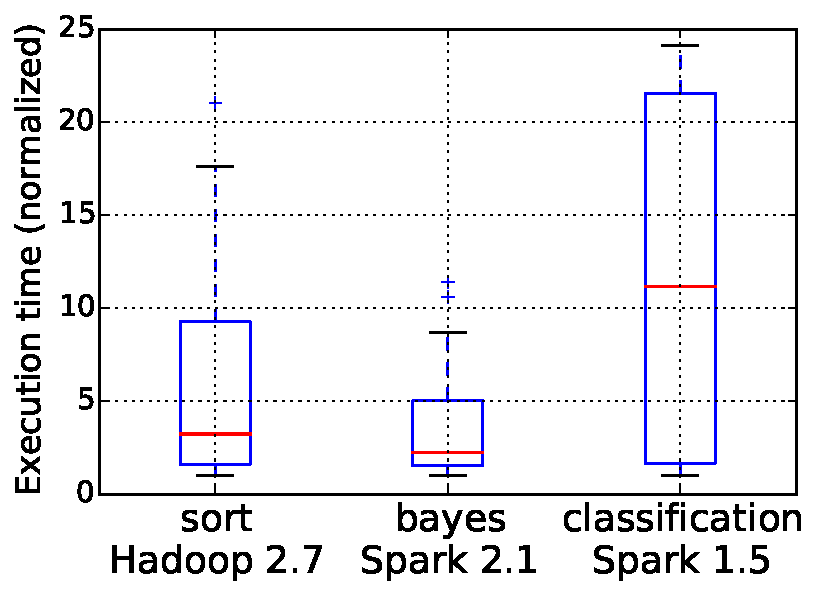
\includegraphics[width=\linewidth]{figures/motivation_bad_choice_time.pdf}
    \caption{Execution time}
    \label{fig:motivation_bad_choice_time}
\end{subfigure}
\hfill
\begin{subfigure}[b]{0.45\textwidth}
    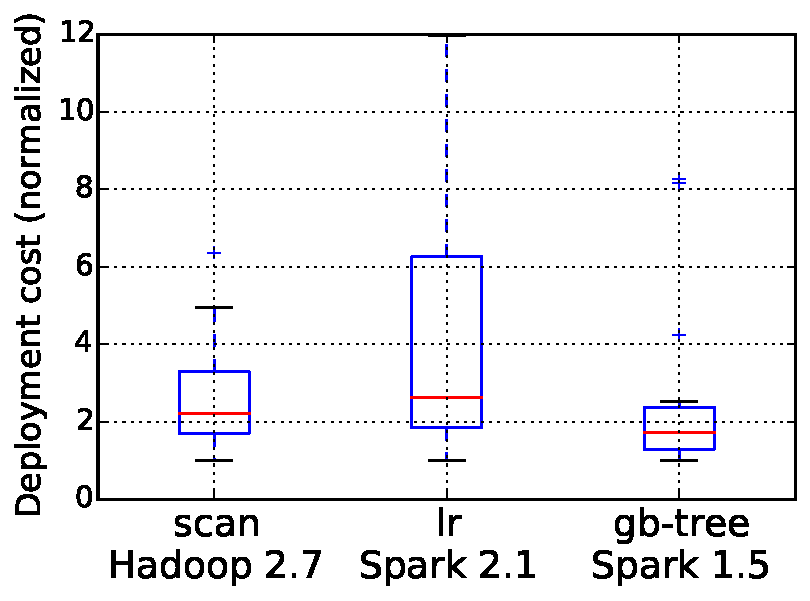
\includegraphics[width=\linewidth]{figures/motivation_bad_choice_cost.pdf}
    \caption{Deployment cost}
    \label{fig:motivation_bad_choice_cost}
\end{subfigure}
\caption{The execution time and deployment cost of workloads running on 18 virtual machines (different types). The execution time of classification-Spark 1.5 in the worst case is 20 times slower that the best VM type. Similarly the deployment cost of running Linear Regression on the worst VM type is 10 times more expensive than the best VM type.}
\label{fig:motivation_bad_choice}
\end{figure}



\subsection*{No VM rules all}
Our empirical data, as shown in \myfigure{\ref{fig:motivation_bad_choice}}, demonstrates that
a bad choice can increase the execution time (of a workload) up to 20 times and can be ten times more costly than the optimal one.
Prior work reports similar results~\cite{Alipourfard2017, Yadwadkar2017}. Careless selection can often end up
with high deployment cost and longer (sub-optimal) execution time.

Even though users are willing to pay a higher cost in exchange for performance, choosing the most expensive VM type may not always result in optimal performance. Figure~\ref{fig:motivation_variance_time} shows the distribution of the execution time when running on the most expensive VM types  (namely c4.2xlarge, m4.2xlarge and r4.2xlarge). For instance, if we look at the distribution of execution times for c4.2xlarge, we observe that c4.2xlarge is the best VM for 50\% of the cases. This means for the other 50\% of the workloads; the most expensive VM type does not guarantee the lowest execution time. We observe similar behavior in Figure~\ref{fig:motivation_variance_cost}, where the least expensive VM, c4.large, does not ensure the lowest deployment cost.

% \myfigure{\ref{fig:motivation_variance_time}} suggests that
% the most expensive VM type can sometimes lead to a ten times slowdown. Possible explanations could be 
% resource bottleneck or resource availability~\cite{Yadwadkar2017}.

% Similarly, when optimizing for cost,
% choosing the cheapest VM type can lead to a higher deployment cost in several cases. \myfigure{\ref{fig:motivation_variance_cost}} shows that the cheapest VM type can increase the deployment cost up to more than eight times.
% Hence, there does not exist an one-size-fits-all VM type.


\begin{figure}
\centering
\begin{subfigure}[b]{0.45\textwidth}
    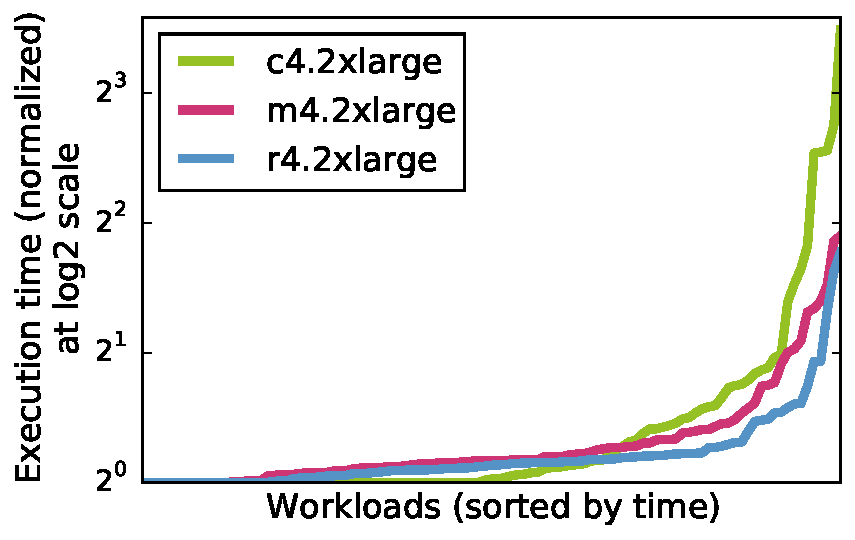
\includegraphics[width=\linewidth]{figures/motivation_variance_time.pdf}
    \caption{Execution time on the most expensive VM types.}
    \label{fig:motivation_variance_time}
\end{subfigure}
\hfill
\begin{subfigure}[b]{0.45\textwidth}
    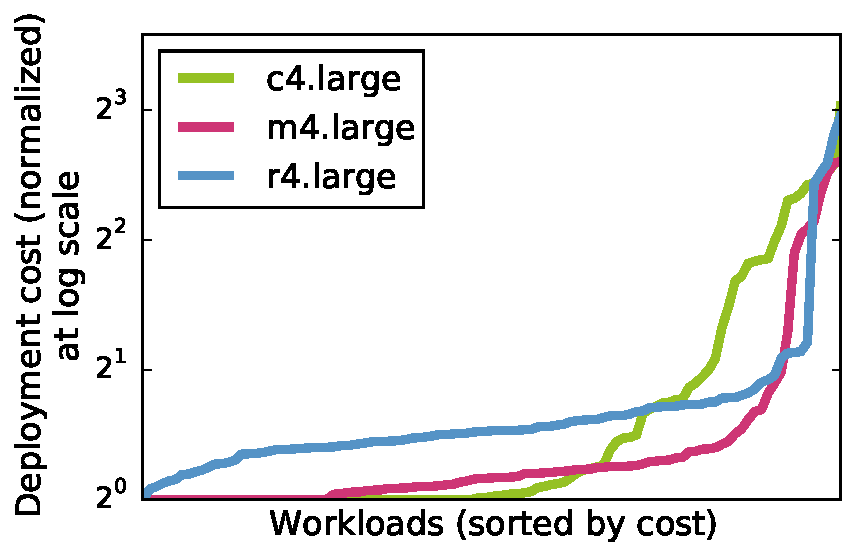
\includegraphics[width=\linewidth]{figures/motivation_variance_cost.pdf}
    \caption{Deployment cost on the least expensive VM types.}
    \label{fig:motivation_variance_cost}
\end{subfigure}
\caption{Performance distribution over different workloads. The performance is normalized to the optimal performance measured in the 18 virtual machines. The \emph{x-axis} represents workloads, sorted by their normalized performance.  Both choosing the most expensive and the cheapest VM types are not desirable.}
\label{fig:motivation_variance}
\end{figure}





\subsection*{The same application with different input sizes favors different VM types}
Machine learning workloads are readily available
such as the machine learning library in Apache Spark and Python~\cite{scikit-learn}.
It is valid to assume that similar workloads would prefer the same VM type provided the user can accurately identify similar workloads.
Consequently, users can always reuse the best VM type for their workloads without testing further.
However, we found that this might not always be the case.
A workload with different input sizes or parameters performs very differently on different VMs~\cite{Venkataraman2016}.
Figure~\ref{fig:motivation_datasize} illustrates how the performance of an application varies with different input sizes.
For example, in Figure~\ref{fig:motivation_datasize_b}
\emph{c4.large} is the most cost-effective VM type for running the \textit{bayes} application with the \emph{small} input size.
However, the deployment cost increases by 40\% (is no longer the optimal VM) when the input size is \emph{large}.
A possible explanation is that a larger input size creates
a resource bottleneck on a smaller VM.
Hence, users need to be more careful
at selecting the best VM type even for the same applications.



\begin{figure}
\centering
\begin{subfigure}[b]{0.45\textwidth}
    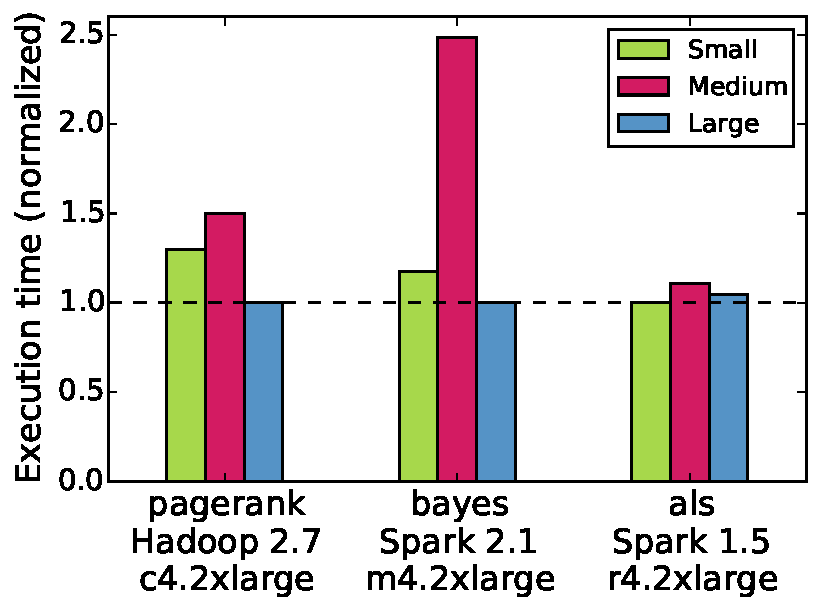
\includegraphics[width=\linewidth]{figures/motivation_datasize_time.pdf}
    \caption{Execution time.}
    \label{fig:motivation_datasize_a}
\end{subfigure}
\hfill
\begin{subfigure}[b]{0.45\textwidth}
    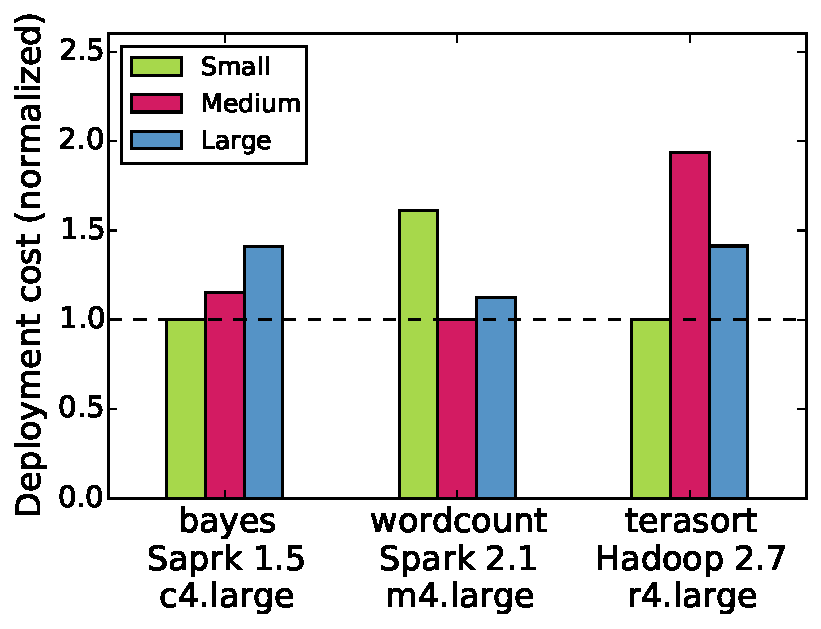
\includegraphics[width=\linewidth]{figures/motivation_datasize_cost.pdf}
    \caption{Deployment cost.}
    \label{fig:motivation_datasize_b}
\end{subfigure}
\caption{Running application with different input sizes result in very different performance.
 The best performing VM types for an application can change when the input size or parameters are changed.}
\label{fig:motivation_datasize}
\end{figure}



\subsection*{Cost creates a level playing field}
Finding a cost-effective VM type can be harder because
a slower VM can be competitive in deployment cost.
In \myfigure{\ref{fig:motivation_variance_time}},  \emph{c4.2xlarge} is the fastest VM type for over 50\% of the workloads (optimal execution time is 1.0).
However in Figure~\ref{fig:motivation_variance_cost}, when considering deployment cost, we observe that
\emph{c4.large} is likely to be a better choice, since it is optimal VM in over 50\% of the workloads.

\myfigure{\ref{fig:level_playing_field}} presents the normalized execution time
and deployment cost of a workload (\emph{regression} on \emph{Spark 1.5}).
The figure demonstrates how execution time can be very different
while deployment cost is similar across all VM types. For example, \emph{m4.large} and \emph{c4.xlarge} are comparable to \emph{c4.2xlarge} in terms of deployment cost.
When the difference between execution times of a workload in different VM types is large, choosing the best VM is easier because there is a clear winner.
Incorporating cost compresses the difference.
Therefore, searching for the most cost-effective VM type becomes more difficult because several inferior choices (in terms of execution time) are now competitive (in deployment cost).
In Section~\ref{sec:comparison}, we show why finding cost-effective VM type
is harder than execution time.


\begin{figure}
    \centering
    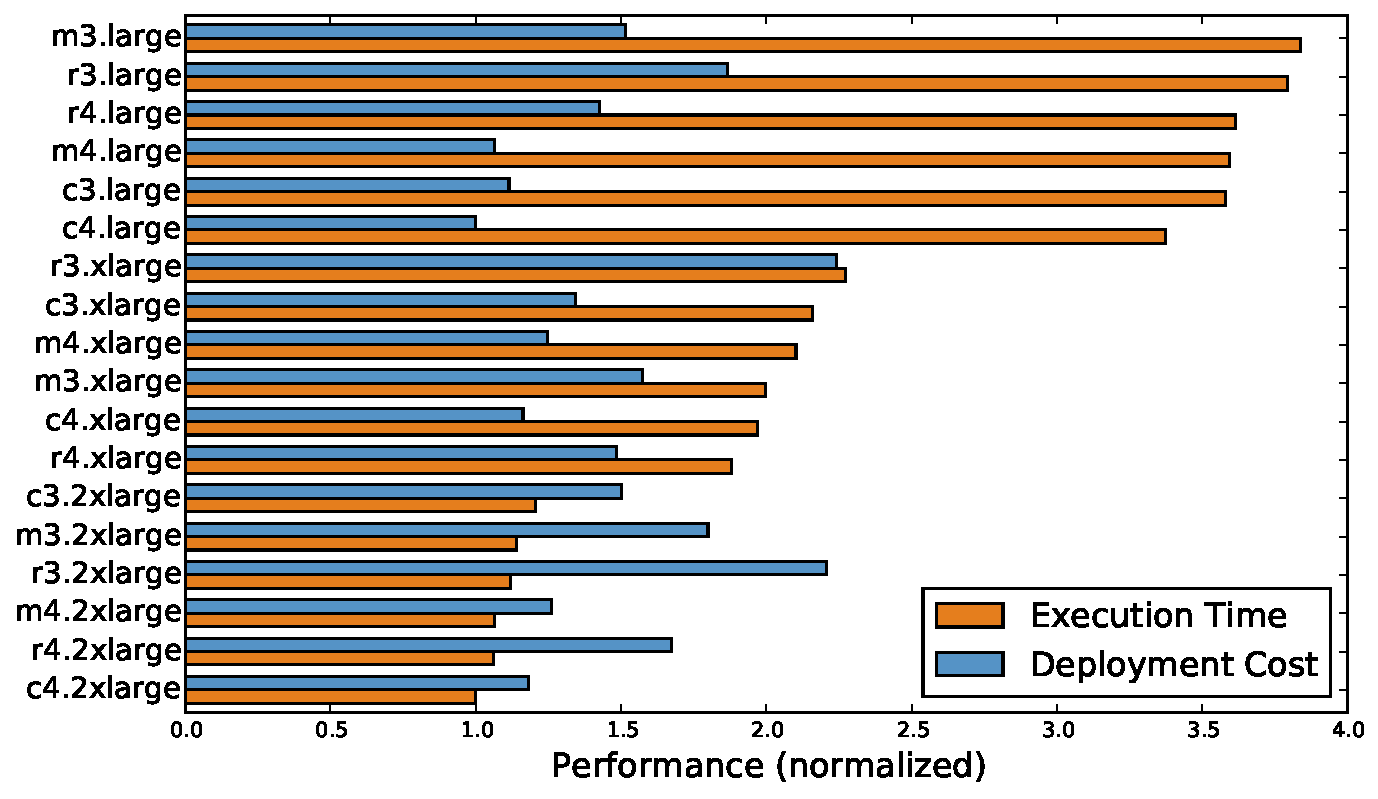
\includegraphics[width=0.8\textwidth]{figures/level_playing_field.pdf}
    \caption{The performance of running the \emph{regression} workload on instances with different VM types.
    Introducing cost creates a \emph{level playing filed}, in which several inferior VM types in execution time are now competitive in deployment cost.
    This observation implies that searching for the most cost-effective configuration is harder than searching for the fastest configuration.}
    \label{fig:level_playing_field}
\end{figure}